%%%%%%%%%%%%%%%%%%%%%%%%%%%%%%%%%%%%%%%%%%%%%%%%%%%%%%%%%%%%
%%% ELIFE ARTICLE TEMPLATE
%%%%%%%%%%%%%%%%%%%%%%%%%%%%%%%%%%%%%%%%%%%%%%%%%%%%%%%%%%%%
%%% PREAMBLE 
\documentclass[9pt,lineno]{elife}
% Use the onehalfspacing option for 1.5 line spacing
% Use the doublespacing option for 2.0 line spacing
% Please note that these options may affect formatting.
% Additionally, the use of the \newcommand function should be limited.


\usepackage{lipsum} % Required to insert dummy text
\usepackage[version=4]{mhchem}
\usepackage{siunitx}
\DeclareSIUnit\Molar{M}

%%%%%%%%%%%%%%%%%%%%%%%%%%%%%%%%%%%%%%%%%%%%%%%%%%%%%%%%%%%%
%%% ARTICLE SETUP
%%%%%%%%%%%%%%%%%%%%%%%%%%%%%%%%%%%%%%%%%%%%%%%%%%%%%%%%%%%%
\title{Sting nematodes modify metabolomic profiles of host plants}

\author[1*,\authfn{1}]{Denis S Willett}
\author[1,\authfn{1}]{Camila C Filgueiras}
\author[2]{Nicole D Benda}
\author[2]{Jing Zhang}
\author[3]{Kevin A Kenworthy}
\affil[1]{Applied Chemical Ecology Technology, Department of Entomology, Cornell AgriTech}
\affil[2]{Entomology and Nemotalogy Department, University of Florida}
\affil[3]{Agronomy Department, University of Florida}

\corr{deniswillett@cornell.edu}{DSW}

\contrib[\authfn{1}]{These authors contributed equally to this work}

%\presentadd[\authfn{3}]{Department, Institute, Country}
% \presentadd[\authfn{4}]{Department, Institute, Country}
% \presentadd[\authfn{5}]{eLife Sciences editorial Office, eLife Sciences, Cambridge, United Kingdom}

%%%%%%%%%%%%%%%%%%%%%%%%%%%%%%%%%%%%%%%%%%%%%%%%%%%%%%%%%%%%
%%% ARTICLE START
%%%%%%%%%%%%%%%%%%%%%%%%%%%%%%%%%%%%%%%%%%%%%%%%%%%%%%%%%%%%

\begin{document}

\maketitle

\begin{abstract}
Please provide an abstract of no more than 150 words. Your abstract should explain the main contributions of your article, and should not contain any material that is not included in the main text.
\end{abstract}


\section{Introduction}

Nematodes, tiny round worms, are ubiquitous denizens of belowground environments.  While many are free-living, the more than 4000 plant parasitic nematodes are devastating in their impacts on human agriculture \cite{jones2013top,moens}. Most important agricultural crops suffer yield loss from plant parasitic nematodes with annual economic damage estimates exceeding \$100 billion \cite{jones2013top, williamson2006nematode}.  

To utilize plants as a resource, plant parasitic nematodes must overcome plant defenses design to thwart nematode feeding.  These defenses range from physical barriers to chemical defenses both inside and outside the plant including toxic root exudates and complex, gene-mediated resistance \cite{yeates1987plants, williamson2006nematode}.  To overcome these defenses

Nematode parasites of plants are world wide...

Parasites overcome plant defences...

Often to overcome plant defenses, close association and coevolution with plant species.  as an example root knot modifies plant defense pathways - endoparasite

Ecto parasites - different lifestyle - do they modify - interaction

metabolomics introduction


introduce case study

close with ecto-endo modification 
and identification of mechanisms of tolerance





\section{Results}

To investigate whether sting nematodes modify metabolite production in their host plants, mixed age \textit{Belonolaimus longicaudatus} nematodes were introduced to the root zones of three African Bermudagrass (\textit{Cynodon transvaalensis}) lines of differing tolerance: one susceptible line (AB03), one moderately tolerant line (AB33), and one tolerant line (AB39).  Comparison control plants received no nematodes.  Ninety days after inoculation,  Plants were unearthed and sting nematode damage assessed.  Following damage assesment, untargeted metabolomic profiling was conducted on root samples.  

\subsection{Bermudagrass responds to sting nematode feeding}
Interestingly, sting nematode populations were significantly (df = 36, t>4, P<0.004, Tukey method) higher on moderately tolerant (AB33) bermudagrass (Figure \ref{fig:figure1}A).  (No sting nematodes were recovered from comparison plants not inoculated with sting nematodes; there was no contamination.)  No significant (df = 36, t = -0.75, P = 0.73) differences in sting nematode populations on susceptible (AB03) or tolerant (AB39) lines were observed.  

Unsurprisingly, presence of sting nematode caused significant (df = 36, t = -9.5, p < 0.0001) reductions in root biomass (Figure \ref{fig:figure1}C).  Despite supporting the highest sting nematode populations, the moderately tolerant line (AB33) showed moderate levels of root biomass loss (Figure \ref{fig:figure1}D). Even though the susceptible line (AB03) supported lower sting nematode populations, it had significantly higher root biomass loss compared to either the moderate (AB33, P = 0.003) or the tolerant (AB39, P < 0.001).  

\subsection{Sting nematodes modify global metabolome of host plants}
These differences are reflected in differences in the global metabolome obtained from root samples.  Experimental factors significantly (x2 = 0.002, df = 5 f = 5.1, p = 0.001) explained 42\% of the observed inertia in the global metabolome by canonical correspondence analysis.  Bermudagrass line (df = 2, X2 = 0.002, F = 8.9, P = 0.001), treatment (nematode inoculation or no nematodes, df = 1, x2 = 0.0001, F = 1.8, P = 0.2), and their interaction (df = 2, x2 = 0.0005, F = 2.9, P = 0.001) significantly resolved groupings in ordination space (Figure \ref{fig:figure2}).  Infection by sting nematode modifies the global metabolome, especially in less tolerant (AB03) and (AB33) lines.

Modifications to the global metabolome are associated with specific compounds.  Indicator species analysis (multi-level pattern analysis) was used to calculate the association of each identified (~5\% of detected compounds) compounds with line and treatment.  L-Pipecolic acid was strongly associated (phi = 0.453, p = 0.001) with plants inoculated with sting nematode.  Abundance of known metabolites across lines was grouped using heirarchical cluster analysis then coupled with association values by line (Figure \ref{fig:figure3}).  Guanine, oxoproline, inosine, and citrulline were closely related and highly associated ( phi >0.51, P <0.003) with the susceptible AB03 line.  A number of compounds were closely associated with the moderately tolerant line AB33 including the closely grouped Orthophosphate, ferrulate, and malate (phi > 0.55, P<0.001). Adenine, sugar alcohols, D-glucaronic acid, asparagine, and theophylline were closely associated (phi>0.52, P<0.001) with the tolerant line (AB39).  


\subsection{Compounds responsible for tolerance to sting nematodes}
To further examine compounds responsible for differences in observed plant responses to sting nematode infection, a metabolome-wide assciation approach was taken using a series of wilcoxon sign-rank contrasts between plants with and without nematodes by line and compound (with correction for the false discovery rate).  Among the compounds detected by this approach, amino acid related compounds seemed to play a large role (Figure \ref{fig:figure4}.  In the most susceptible line (AB03), amino acid abundance was significantly (p< 0.05) suppressed in seven out of the 13 amino acid compounds assayed.  Four of the remaining compounds (L-isoleucine, L methionione, citrulline, and n-alpha ...) showed similar, albeit non-significant, trends.  This pattern was not apparent in either the moderately susceptible (AB33) nor tolerant (AB39) lines.  

In addition to sting nematodes modifying amino acid production in susceptible bermudagrass plants, production of a number of defence-related compounds was associated with nematode abundance.  Higher normalized levels of D-Glucaronic acid, Glycolate, and Phenylalanine were significantly (r2 = 0.24, 0.21, 0.23; P = 0.035, 0.049, 0.38 respectively) associated with lower levels of sting nematode (Figure \ref{fig:figure5}A-C).  Although lines had differing levels of Phenylalanine and nematodes, the negative relationship (slope of -89.6, t = -2.1, P = 0.05) was apparent within lines (Figure \ref{fig:figure5}D).  

Differences in L-Pipecolic Acid were also strongly associated with sting nematode presence. L-Pipecolic acid production significantly (t = 2.74, df = 12, P = 0.05 after conservative bonferroni correction) increased in the presence of sting nematode in the tolerant (AB39) line (Figure \ref{fig:figure6}A).  Although there were no within-line trends, lines (particularly the tolerant AB39) with increased production had substantially reduced sting nematode populations (Figure \ref{fig:figure6}B). Although not significant at p= 0.05, the susceptible line followed trends of increased L-pipecolic acid and reduced nematode population (Figure \ref{fig:figure6}A,B).  

\section{Discussion}


\section{Methods and Materials}


\subsection{Organisms}

Three African Bermudagrass (\textit{Cynodon transvaalensis} Burtt-Davy) lines were used to evaluate metabolomic responses to pathogen infection.  One susceptible line (AB03), one tolerant line (AB39), and one line with moderate tolerance (AB33) were stolon propagated and allowed to establish for 30 days in 4cm diameter, 30cm deep UV-stabilized Ray Leach Cone-tainers filled with USGA grad sand followed with a soil plug (to prevent sand leakage). Plants were grown in a climate controlled greenhouse at 25C and 50\% RH under a 11:13 light:dark cycle.  Plants were watered twice daily for 5 minutes and received 24-8-16 NPK liquid fertilizer on a weekly basis.  Sting nematode (\textit{Belonolaimus longicaudatus} Rau) originally collected from Florida turf and reared on \textit{C. transvaalensis} were used in bioassays. 

\subsection{Bioassays}

To evaluate the effects of nematode infection on bermudagrass metabolite response, treated plants in conetainers were inoculated with 50 sting nematodes of mixed age and gender per conetainer.  Control (uninoculated) plants did not receive any nematode treatment. Seven replications of each line (AB03, AB33, AB39) and treatment (inoculated, uninoculated) combination were conducted.  Ninety days following nematode inoculation (time enough for nematode growth and reproduction), plants were removed from the conetainer, the soil plug removed, and the sand gently rinsed to extract the nematodes for further processing through centrifugal flotation and counting on an inverted microscope.  Rinsed roots were placed in 50ml falcon tubes then immersed in liquid nitrogen and stored at -80 C until lyophilization.  Lyophilzed roots were weighed and samples selected for metabolomics analysis. 

\subsection{Metabolomics}

Following weighing the entire root biomass, 0.5 gram root samples were transferred to 2ml centrifuge tubes and ground in a Geno/Grinder 2010 tissue homogenizer with ball bearings.  After grinding, metabolites were extracted through addition of 1.5ml of 1:1 Methanol:Ammonium Acetate, addition of 20ul internal standard mix, vortexing, and centrifugation at 17,000G for 10 minutes.  Following centrifugation, 800ul of supernatant was transfered to an LC vial and 1ul introduced to a Thermo Scientific Dionex Ultimate 3000 UHPLC using reverse phase chromatography with a ACE Excel 2 C18-PFP (100 x 2.1mm, 2um) at 25C and a flow rate of 350ul/min.  ....Solvent Gradient Here.... 

Following separation by liquid chromatography, samples were introduced to a Thermo Q-Exactive Orbitrap mass spetrometer.  All samples were analyzed in positive and negative heated electrospray ionization with a mass resolution of 35,000 at m/z 200 using polarity switching....More details.  


\subsection{Analysis}

\subsubsection{Bioassays}

The effects of bermudagrass line, treatment, and their interaction on observed nematode counts were model using linear models and analysis of variance.  Residual diagnostics were consulted to ensure conformity of assumptions of normality and homoscedasticity while model significance, likelihood ratios, information criteria, coefficient of determination, and residual examination were used to select the best fit models.  Post-hoc comparisons were evaluated using Tukey's method for controlling the family-wise error rate. 

Similarly, the effects of bermudagrass line, treatment, nematode count, and their interaction on observed root weights were modeled using linear models and analysis of variance. Residual diagnostics were consulted to ensure conformity of assumptions of normality and homoscedasticity while model significance, likelihood ratios, information criteria, coefficient of determination, and residual examination were used to select the best fit models.  Outliers were identified and removed through visual examination of residual diagnostics (including QQ-Plots, Cook's Distance, and Leverage) and mean-shift outlier tests.  Post-hoc comparisons were evaluated using Tukey's method for controlling the family-wise error rate.

Root biomass loss estimation was accomplished through non-parametric bootstrapping (with 1000 replications) to estimate the difference in root biomass between bermudagrass plants inoculated with sting nematode and uninoculated plants.  Differences between median root loss were evaluated with one-sided permutation tests and adjusted using Bonferroni's method for controlling the family-wise error rate.


\subsubsection{Metabolomics}

Raw mass spectrometry data were exported and uploaded to Metabolomics Workbench (Study ID ST000353).  In preparation for analysis, known compounds with more than one retention time were collapsed into a single known compound.  Additionally, contaminants and internal standards were removed from future analysis (Appendix A for list of contaminants and standards removed).  Following cleaning, missing data (less than 8.3\% per sample) were imputed using a k-nearest neighbors approach (k = 5).  Following imputation, data were normalized using variance stabilizing normalization (li et al) to adjust for between-run variations.  

To determine whether there were differences between line and nematode treatment, canonical correspondence analysis was applied to the global metabolome (both known and unidentified compounds).  Results from the canonical correspondence analysis were further evaluated with permutational analysis of variance with 1000 permutations. Line, treatment, and their interaction were evaluated for their effect on the observed metabolomic profiles.  The best fit model was chosen based on permutation statistics (permuted F scores), coefficient of determination, deviance metrics, and goodness of fit metrics.  

To examine relationships between labeled metabolites and lines, heirarchical cluster analysis was used to group compounds with similar abundances across lines.  Indicator species analysis (multi-level pattern analysis) was then used to explore associations of each labeled compound with lines and treatment using Pearson's Phi coefficient of association as the metric. 

To examine differences in abundance of individual labeled compounds, a metabolome wide association study approach was taken where Wilcoxon tests were applied to each compound by line to evaluate differences in compound abundance between uninoculated plants without nematodes and inoculated plants infected by nematodes.  Resultant P values were corrected for the false discovery rate using the Benjami and Hochberg method.  

To further explore the effect of individual compounds on nematode abundance, compounds of interest from the indicator species analysis and metabolome wide association were evaluated for their relationship to observed nematode population levels.  To do so, abundances and nematode counts were normalized by line to account for differences between genotypes then evaluated with linear models to determine the effect of normalized compound abundance on normalized nematode presence. Model fits were evaluated with information criteria, residual examination, model significance, and coefficient of determination.  


\subsubsection{Data Management}

Raw LC/mass spectrometry data were uploaded to metabolomics workbench.  All analysis on the raw data was conducted in R version 3.5.2 using RStudio as an IDE (with Vim keybindings).  A full list of packages used to facilitate the analysis can be found in Appendix E.  All code, including dockerfiles and manuscript documentation, is available on GitHub (...).  








Guidelines can be included for standard research article sections, such as this one. 

\lipsum[3]

\section{Some \LaTeX{} Examples}
\label{sec:examples}

Use section and subsection commands to organize your document. \LaTeX{} handles all the formatting and numbering automatically. Use ref and label commands for cross-references.

\subsection{Figures and Tables}

\begin{figure}
\begin{fullwidth}
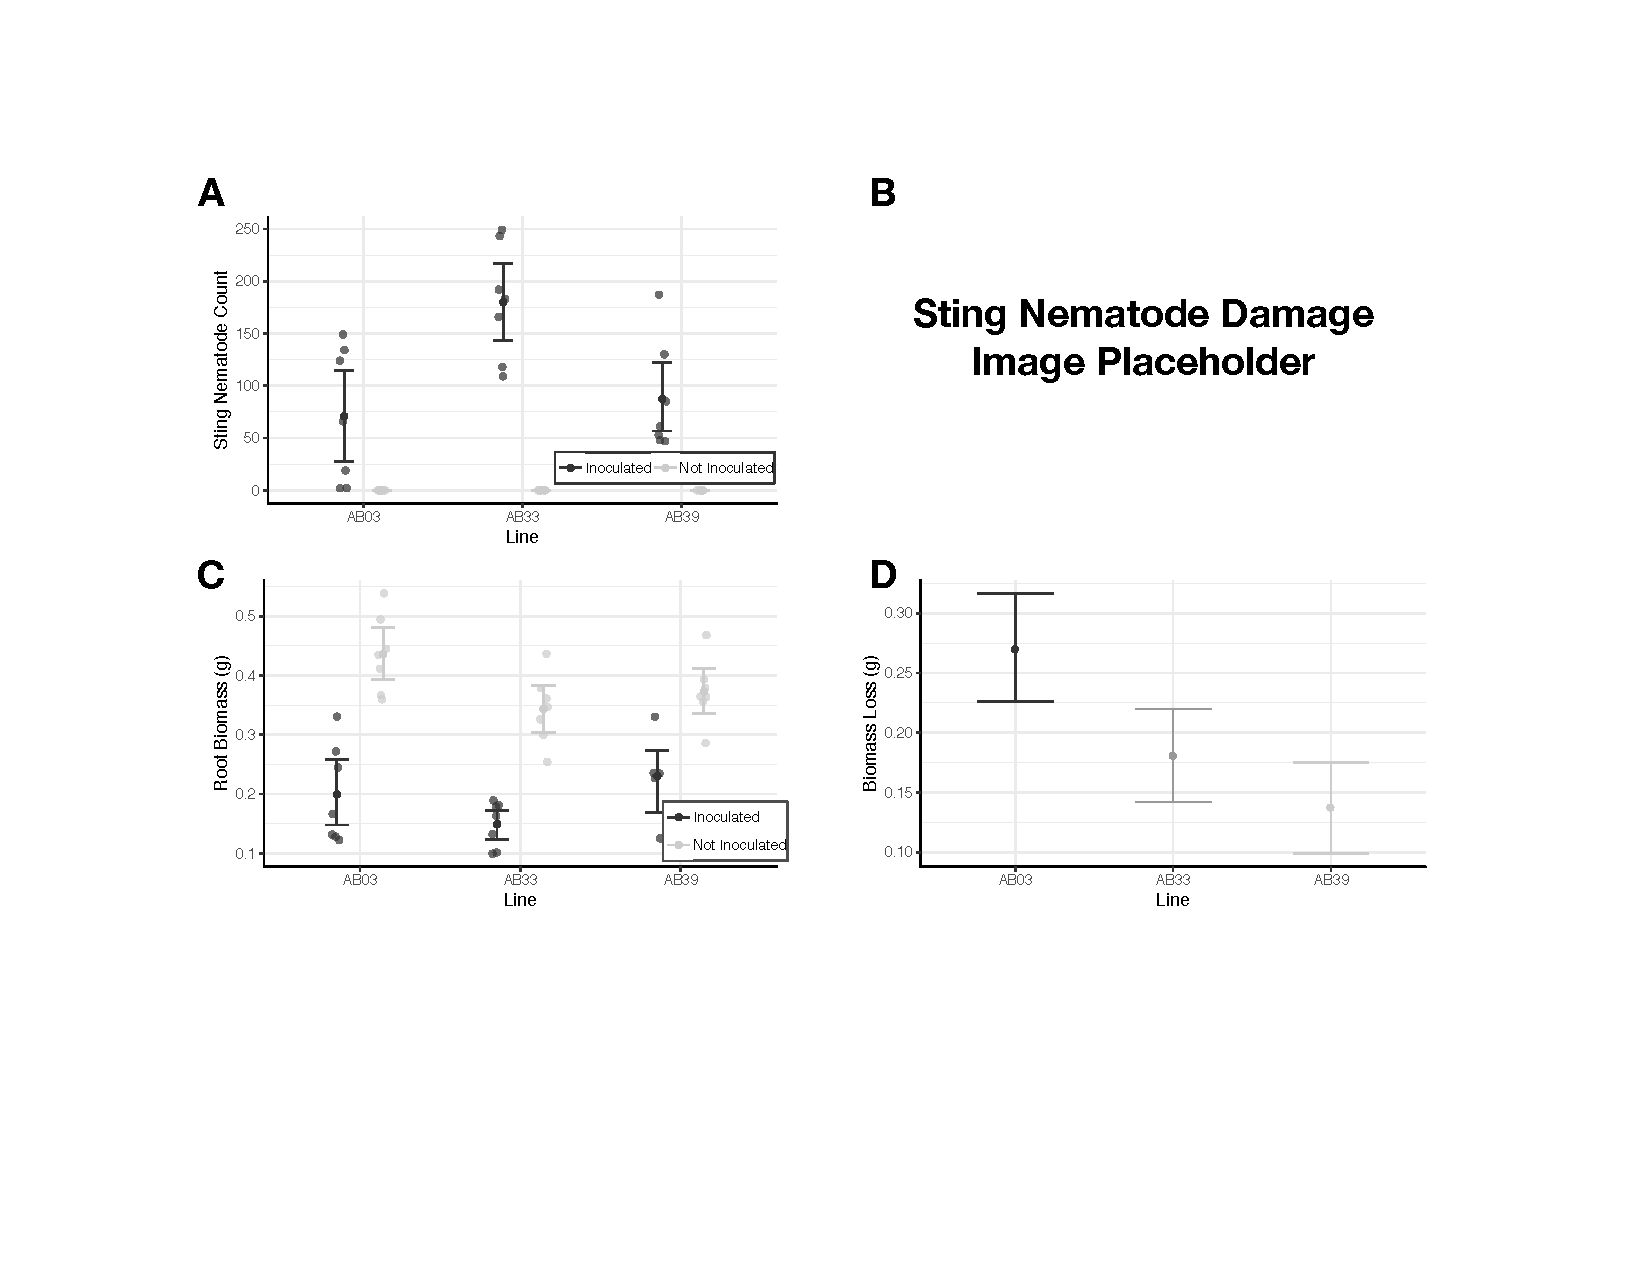
\includegraphics[width=0.95\linewidth]{figures/publication_figures/figure-1.pdf}
\caption{Sting nematode (\textit{Belonolaimus longicaudatus}) response to three different lines of bermudagrass.  A) Counts of sting nematodes recovered from the roots of bermudagrass 90 days after inoculation.  B) Bermudagrass root damage from sting nematode.  C) Root biomass of inoculated and uninoculated bermudagrass.  D) Loss of bermudagrass root biomass due to infection by sting nematode.  In A and C, transparent points are raw observations while solid points and error bars represent mean and bootstrapped 95\% confidence intervals respectively.  In D, points and error bars represent median bootstrapped root loss and bootstrapped 95\% confidence intervals respectively.   }
\label{fig:figure1}
\end{fullwidth}
\end{figure}


\begin{figure}
\begin{fullwidth}
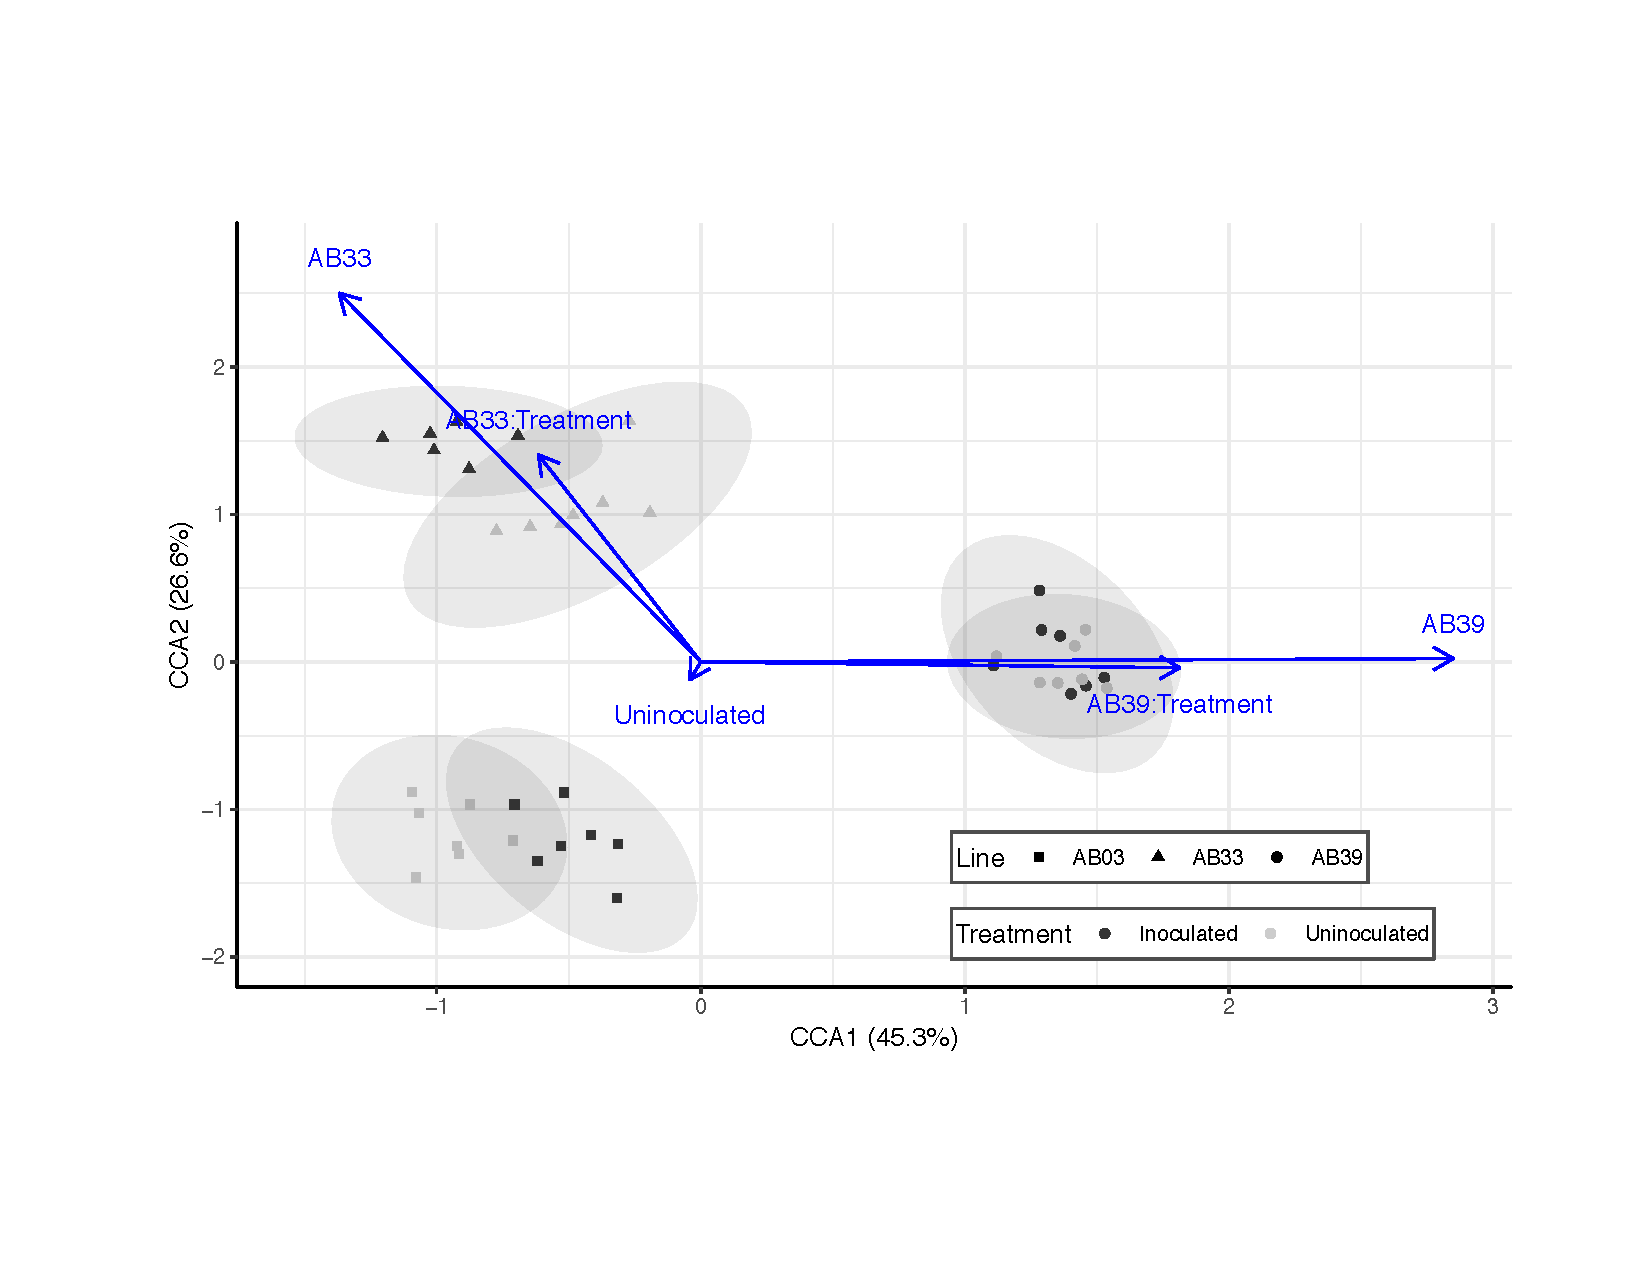
\includegraphics[width=0.95\linewidth]{figures/publication_figures/figure-2.pdf}
\caption{Differences in global metabolome of three bermudagrass lines inoculated and uninoculated with sting nematode.  Axes represent first two orthogonal axes from canonical correspondence analysis with percentages indicating relative contribution of each axis to constrained $\chi^2$.  Points represent the metabolome of individual bermugrass replicates projected into ordination space.  Ellipses are 95\% confidence intervals for each treatment-line combination.  Blue arrows represent explanatory variables; direction of arrow depicts direction of the gradient while length denotes relative (scaled) importance.  }
\label{fig:figure2}
\end{fullwidth}
\end{figure}


\begin{figure}
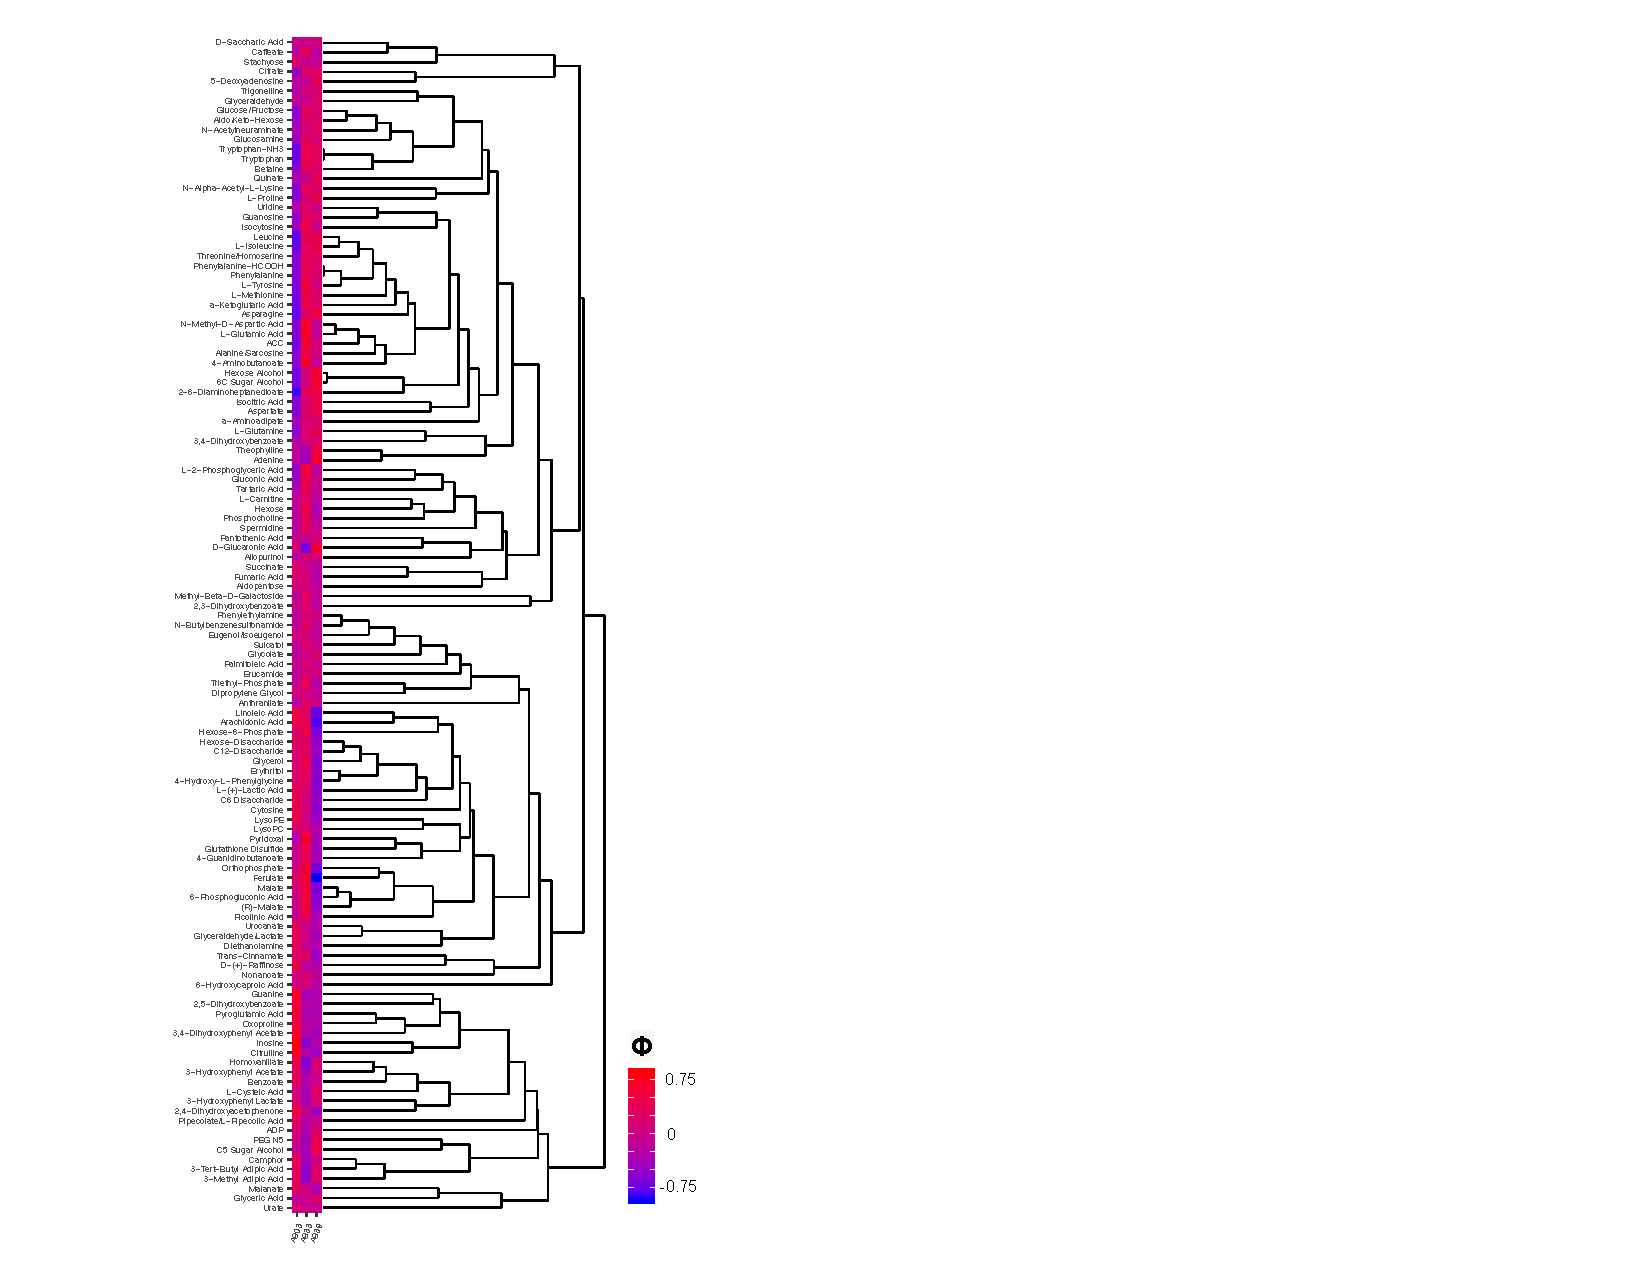
\includegraphics[height = 9in]{figures/publication_figures/figure-3.pdf}
\caption{Known compounds associated with each of three bermudagrass lines.  Values are Pearson's $\phi$ coefficient of association.  Higher (darker red) indicates compounds are more closely associated with that line.  }
\label{fig:figure3}
\end{figure}

\begin{figure}
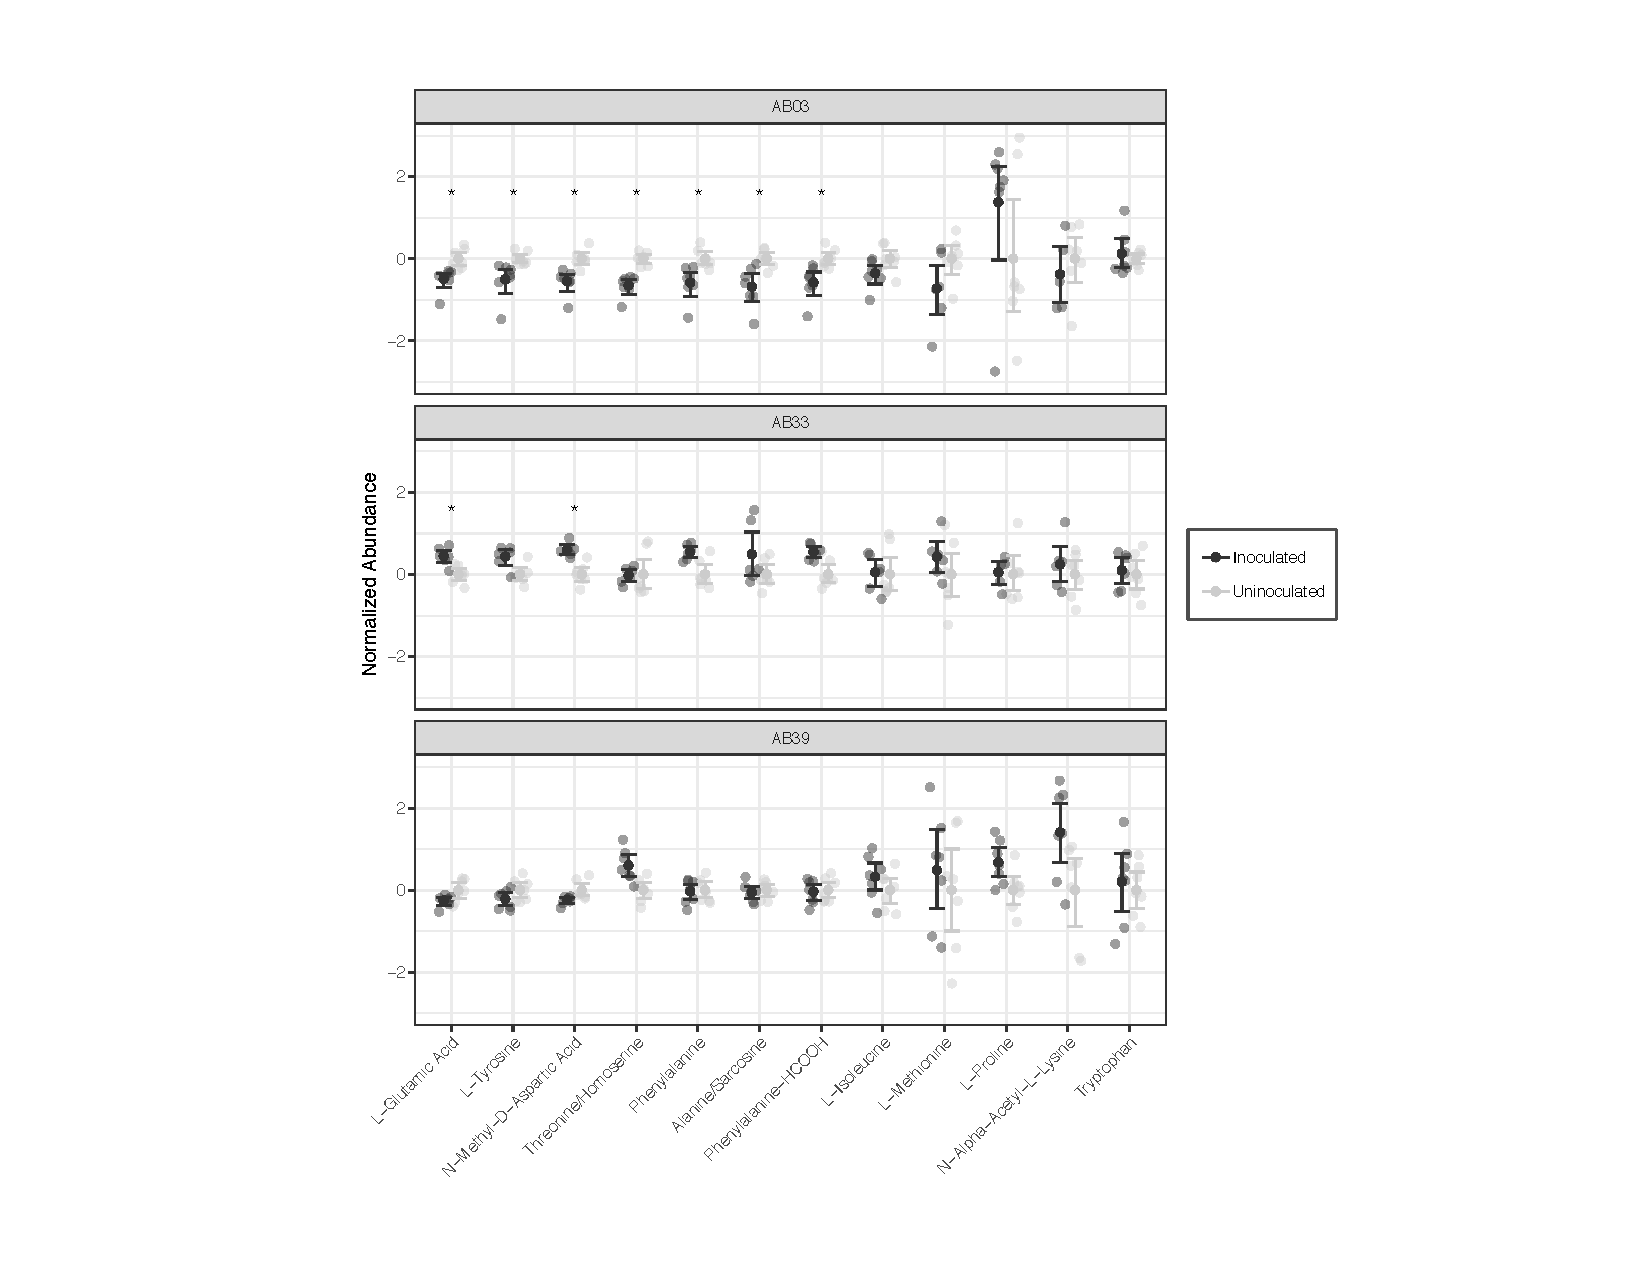
\includegraphics[width = 0.95\linewidth]{figures/publication_figures/figure-4.pdf}
\caption{Normalized abundances of amino acid related compounds across three different bermudagrass lines inoculated and not-inoculated with sting nematode.  Abundances are normalized by compound and line to facilitate visual comparison.  Transparent points are individual observations; solid points and error bars denote mean and 95\% bootstrapped confidence intervals respectively.  Significant difference between plants with and without sting nematode are denoted by asterisks and was determined by Wilcoxon Sign Rank tests on non-normalized abundances with correction for the false discovery rate.  }
\label{fig:figure4}
\end{figure}


\begin{figure}
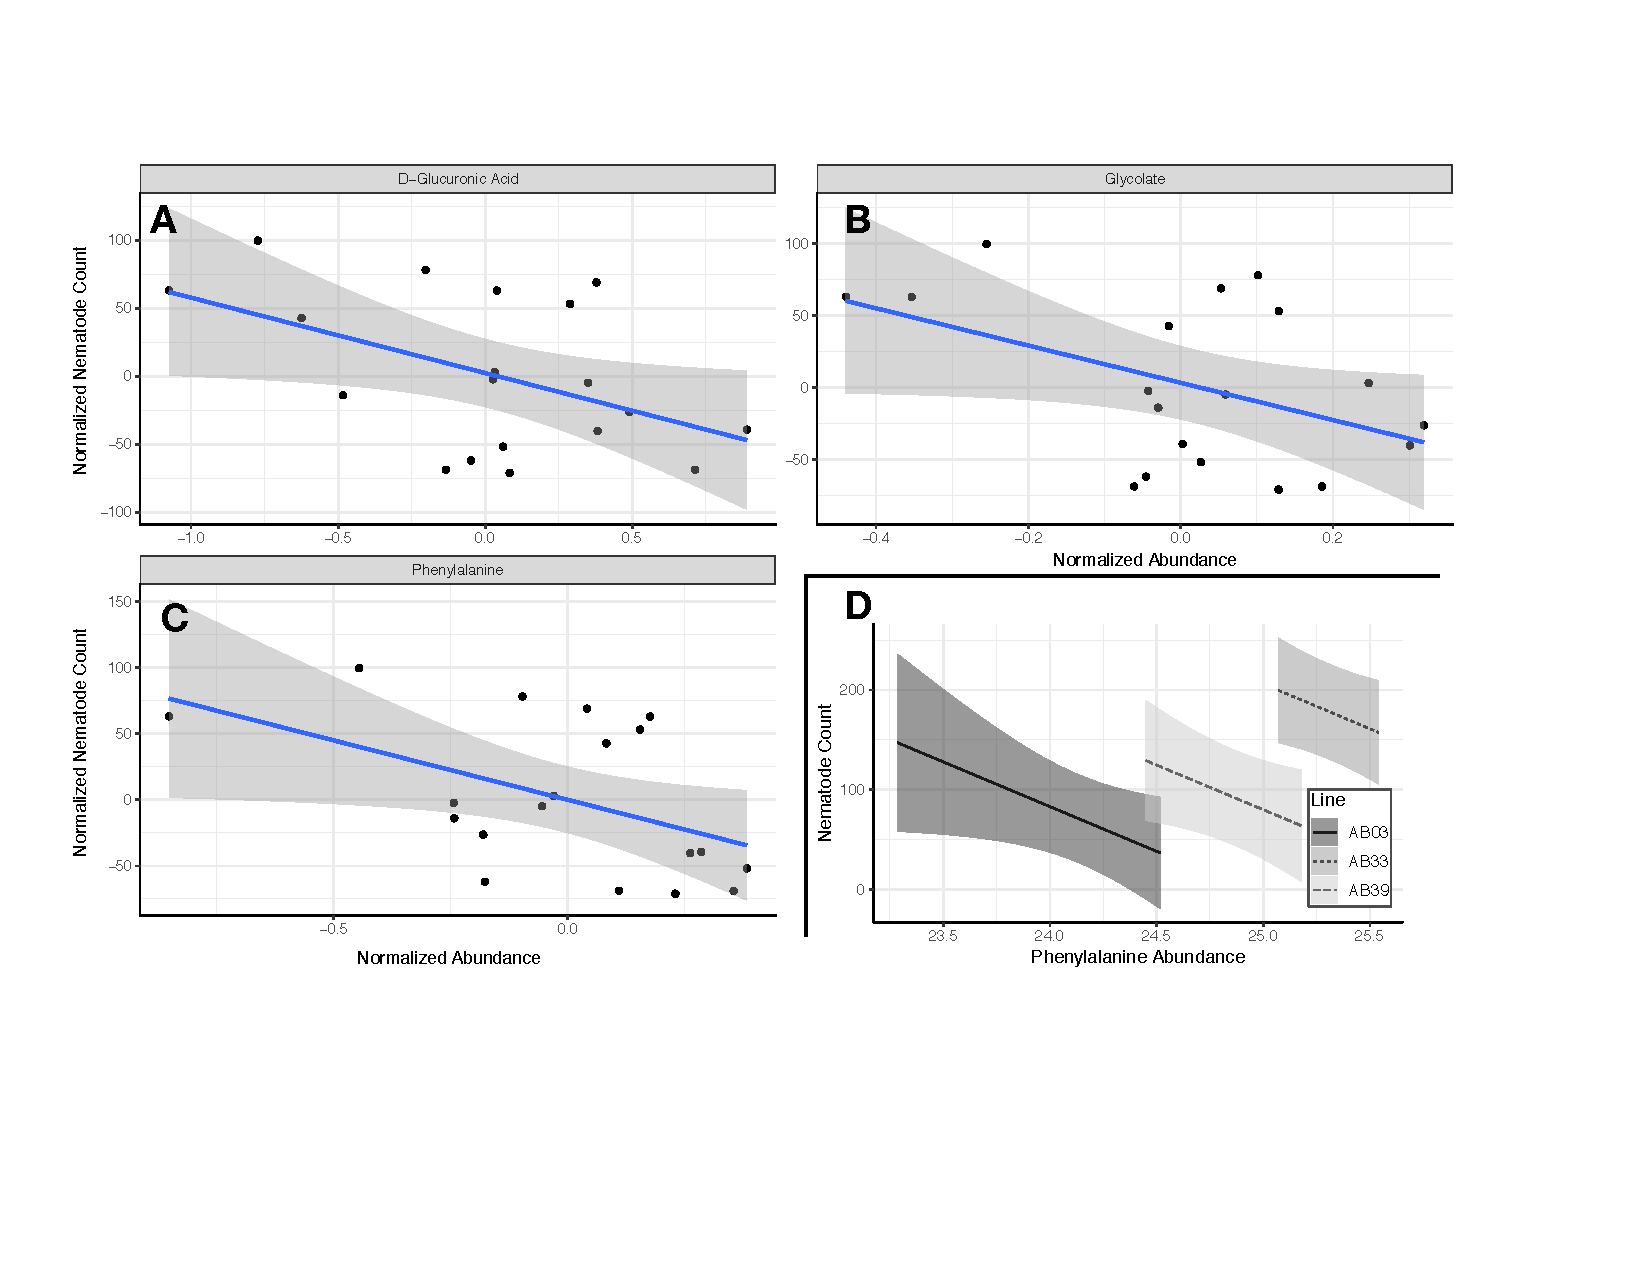
\includegraphics[width = 0.95\linewidth]{figures/publication_figures/figure-5.pdf}
\caption{A,B,C) Relationships between important metabolites and nematode abundance.  Abundances and nematode counts were normalized to facilitate comparison across lines.  Points denote individual observations while blue lines and shaded areas denote linear model fits (all significant at $P < 0.05$ with $R^2$ greater than 0.2.  D) Modeled relationship between observed nematode counts and phenylalanine abundance (not normalized by line).  Lines represent modeled relationship across range of observed phenylalanine abundances with shaded areas denoting 95\% confidence intervals. }
\label{fig:figure5}
\end{figure}

\begin{figure}
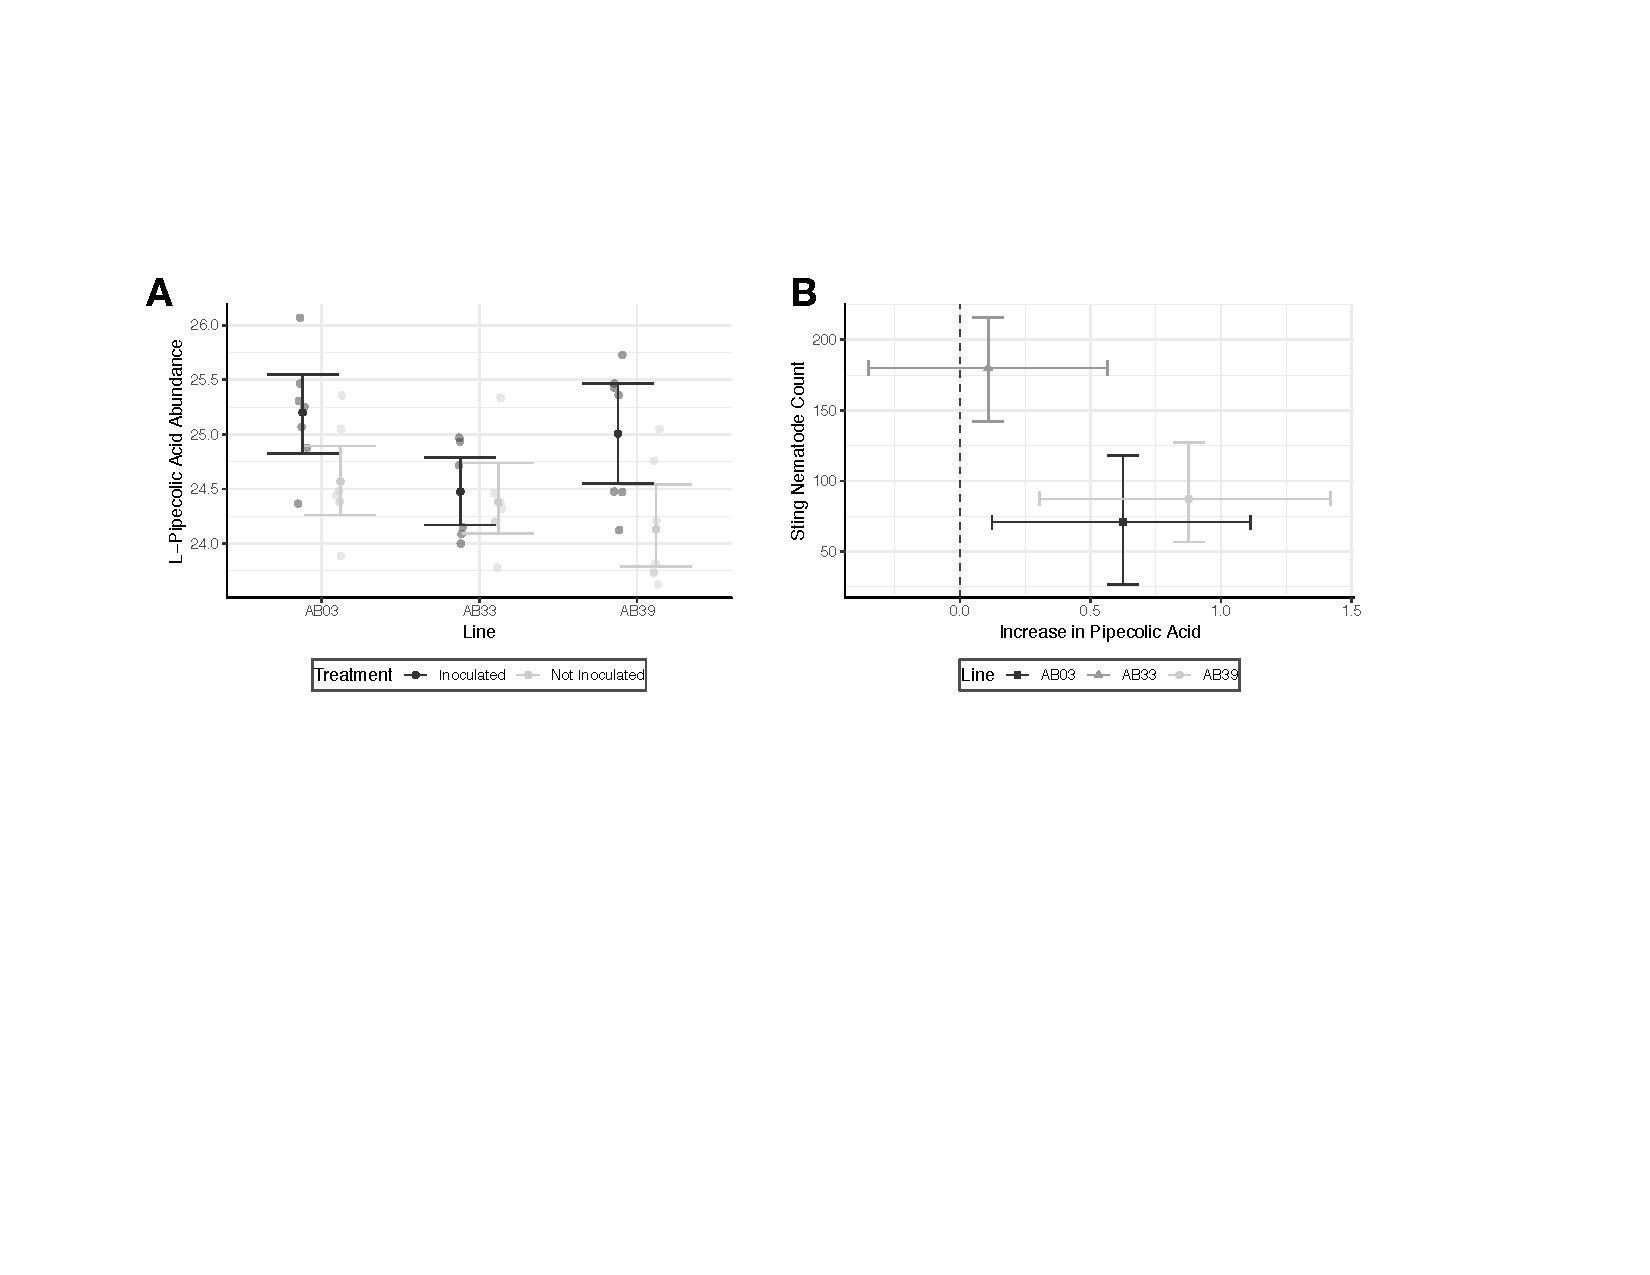
\includegraphics[width = 0.95\linewidth]{figures/publication_figures/figure-6.pdf}
\caption{A) L-Pipecolic Acid production in bermudagrass inoculated and not inoculated with sting nematode.  Transparent points indicate observed values.  Solid points and error bars indicate means and bootstrapped 95\% confidence intervals respectively.  B) Relationship between increases in L-Pipecolic Acid (difference between inoculated and not inoculated plants) and observed Sting nematode counts on bermudagrass roots.  Points and error bars indicate mean and bootstrapped 95\% confidence intervals respectively.   }
\label{fig:figure6}
\end{figure}






\subsection{Citations}

LaTeX formats citations and references automatically using the bibliography records in your .bib file, which you can edit via the project menu. Use the \verb|\cite| command for an inline citation, like \cite{Aivazian917}, and the \verb|\citep| command for a citation in parentheses \citep{Aivazian917}. The LaTeX template uses a slightly-modified Vancouver bibliography style. If your manuscript is accepted, the eLife production team will re-format the references into the final published form. \emph{It is not necessary to attempt to format the reference list yourself to mirror the final published form.} Please also remember to \textbf{delete the line} \verb|\nocite{*}| in the template just before \verb|\bibliography{...}|; otherwise \emph{all} entries from your .bib file will be listed! 

\begin{featurebox}
\caption{This is an example feature box}
\label{box:simple}
This is a feature box. It floats!
\medskip

\includegraphics[width=5cm]{example-image}
\featurefig{`Figure' and `table' captions in feature boxes should be entered with \texttt{\textbackslash featurefig} and \texttt{\textbackslash featuretable}. They're not really floats.}

\lipsum[1]
\end{featurebox}

\subsection{Mathematics}

\LaTeX{} is great at typesetting mathematics. Let $X_1, X_2, \ldots, X_n$ be a sequence of independent and identically distributed random variables with $\text{E}[X_i] = \mu$ and $\text{Var}[X_i] = \sigma^2 < \infty$, and let
\begin{equation}
\label{eq:CLT}
S_n = \frac{X_1 + X_2 + \cdots + X_n}{n}
      = \frac{1}{n}\sum_{i}^{n} X_i
\end{equation}
denote their mean. Then as $n$ approaches infinity, the random variables $\sqrt{n}(S_n - \mu)$ converge in distribution to a normal $\mathcal{N}(0, \sigma^2)$.

\lipsum[3] 

\begin{figure}
\includegraphics[width=\linewidth]{elife-13214-fig7}
\caption{A text-width example.}
\label{fig:view}
%% If the optional argument in the square brackets is "none", then the caption *will not appear in the main figure at all* and only the full caption will appear under the supplementary figure at the end of the manuscript.
\figsupp[Shorter caption for main text.]{This is a supplementary figure's full caption, which will be used at the end of the manuscript.}{\includegraphics[width=6cm]{frog}}\label{figsupp:sf1}
\figsupp{This is another supplementary figure.}{\includegraphics[width=6cm]{frog}}
\videosupp{This is a description of a video supplement.}\label{videosupp:sv1}
\figdata{This is a description of a data source.}\label{figdata:first}
\figdata{This is another description of a data source.}\label{figdata:second}
\end{figure}

\subsection{Other Chemistry Niceties}

You can use commands from the \texttt{mhchem} and \texttt{siunitx} packages. For example: \ce{C32H64NO7S}; \SI{5}{\micro\metre}; \SI{30}{\degreeCelsius}; \SI{5e-17}{\Molar}

\subsection{Lists}

You can make lists with automatic numbering \dots

\begin{enumerate}
\item Like this,
\item and like this.
\end{enumerate}
\dots or bullet points \dots
\begin{itemize} 
\item Like this,
\item and like this.
\end{itemize}
\dots or with words and descriptions \dots
\begin{description}
\item[Word] Definition
\item[Concept] Explanation
\item[Idea] Text
\end{description}

Some filler text, because empty templates look really poorly. \lipsum[1]


\section{Acknowledgments}

Additional information can be given in the template, such as to not include funder information in the acknowledgments section.

\nocite{*} % This command displays all refs in the bib file. PLEASE DELETE IT BEFORE YOU SUBMIT YOUR MANUSCRIPT!
\bibliography{elife-sample}

%%%%%%%%%%%%%%%%%%%%%%%%%%%%%%%%%%%%%%%%%%%%%%%%%%%%%%%%%%%%
%%% APPENDICES
%%%%%%%%%%%%%%%%%%%%%%%%%%%%%%%%%%%%%%%%%%%%%%%%%%%%%%%%%%%%

\appendix
\begin{appendixbox}
\label{first:app}
\section{Firstly}
\lipsum[1]

%% Sadly, we can't use floats in the appendix boxes. So they don't "float", but use \captionof{figure}{...} and \captionof{table}{...} to get them properly caption.
\begin{center}
\includegraphics[width=\linewidth,height=7cm]{frog}
\captionof{figure}{This is a figure in the appendix}
\end{center}

\section{Secondly}

\lipsum[5-8]

\begin{center}
\includegraphics[width=\linewidth,height=7cm]{frog}
\captionof{figure}{This is a figure in the appendix}
\end{center}

\end{appendixbox}

\begin{appendixbox}
\includegraphics[width=\linewidth,height=7cm]{frog}
\captionof{figure}{This is a figure in the appendix}
\end{appendixbox}
\end{document}
